\chapter{Theory and recent work}

\section{Recent work}

Most of the recent work in object detection and recognition revolves around the need to speed up detection phase of recognition pipeline. One of the most advancement in this area was made by introducing \rcnn{} type of networks, in three iterations -- \rcnn~\cite{rcnn}, Fast \rcnn~\cite{fast} and Faster \rcnn~\cite{faster}. R in \rcnn{} stands for Regions to illustrate combination of region proposals with convolutional neural network. The main progress made in last iteration of \rcnn{} (Faster) was introduction of RPN units. RPN unit is a Region Proposal Network which takes care of proposing regions of interest for convolutional network while sharing the weights and computation with convolutional network used for recognition. Such RPN can be made to output limited number of proposals in scene and original paper reported that 300 was the most suitable number -- therefore we were using only 300 as well.

Another difficulty which we were facing was domain shift. Since our goal was to have an easily trainable system, which could be potentially used for different training and testing domain (namely generated data used as training domain with real data used as testing domain), it was needed to adopt some techniques necessary to overcome such domain shift. However, due to time restrictions we were only able to use simple re-training, which was recently shown by Rozantsev~\cite{shift} might be insufficient when compared to more recent techniques. Rozantsev was using simple means of having two concurrent networks running next to each other while sharing the weights between some layers and allowing slight transformation between other layers which rendered to be superior to other techniques previously used to overcome domain shift.

Another important question was which of the convolutional network frameworks to use. While Caffe~\cite{caffe} seemed to be most reasonable choice mostly because Faster \rcnn{} was implemented using Caffe, we also considered using other frameworks such as TensorFlow~\cite{tensorflow} by Google or Theano~\cite{theano}. However, when using Theano, we would most likely have to write significantly larger amount of code though with more control over it since Theano is only compiler of mathematic expressions. Ultimately we chose Caffe for two reasons -- it still has a lot more support in scientific community than TensorFlow and implementation of Faster \rcnn{} work was built around it.

\section{Theory}

\subsection{Convolutional neural network}
\def\nsep{2.5cm}

The problem of object detection and recognition is one of the oldest in the field of computer vision. The object detection deals with finding the objects of interest in a scene where the multiple objects can be present at once, while the object recognition tries to classify either objects extracted by object detection tools or the whole image. The object detection problem is inherently much more difficult than object recognition since objects can be present in an image in vast amount of various locations, scales or different aspect ratios. One of the approaches used for object recognition is using convolutional neural networks.

The reasoning behind this is rather simple. Since artificial neurons are trying to simulate actions of real neurons in brain, using a convolutional network is next logical step because it is believed processing images in our brain relies on connecting visual information from close surroundings together, much like convolutional filters do.

\begin{figure}
\begin{tikzpicture}[shorten >=1pt,->,draw=black!50]
\tikzstyle{neuron}=[circle,fill=ctulightblue,minimum size=17pt,inner sep=0pt]
\tikzstyle{input neuron}=[neuron, fill=white!50]
\tikzstyle{every pin edge}=[<-,shorten <=1pt]
\foreach \y in {1,...,3}
	\node[input neuron] (I-\y) at (0,-\y) {$\textbf{x}_\y$};
\node[input neuron] (I-5) at (0,-4) {\vdots};
\node[input neuron] (I-4) at (0,-5) {$\textbf{x}_n$};
\node[neuron] (B) at (\nsep,-1) {$\theta$};
\node[neuron] (N) at (\nsep,-3) {$\sum$};
\foreach \s in {1,...,3}
	\path (I-\s) edge node[above] {$\textbf{w}_\s$} (N);
\path (I-4) edge node[above] {$\textbf{w}_n$} (N);
\path (B) edge node[left] {$\textbf{w}_0$} (N);
\node[neuron] (A) at (2*\nsep, -3) {$\phi(\cdot)$};
\node[input neuron] (O) at (3*\nsep, -3) {$o(\textbf{x})$};
\path (N) edge (A);
\path (A) edge (O);
\end{tikzpicture}
\caption{Structure of artificial neuron}
\label{aneuron}
\end{figure}

The artificial neuron itself (shown on figure \ref{aneuron}) is described by the equation $o(\textbf{x}) = \phi(\textbf{x}^{\top}\textbf{w} + \textbf{w}_0\theta)$, where $\phi(\cdot)$ is a usually non-linear activation function, $\textbf{w}$ is a weight vector associated with a given neuron, $\theta$ is a so called bias of a neuron and $\textbf{x}$ is the input vector fed into neuron. If we start connecting these neurons next to each other and then into layers, we get fully-connected neural networks (shown on figure \ref{nnet}).

\begin{figure}
\begin{tikzpicture}[shorten >=1pt,->,draw=black!50, node distance=\nsep]
    \tikzstyle{every pin edge}=[<-,shorten <=1pt]
    \tikzstyle{neuron}=[circle,fill=black!25,minimum size=17pt,inner sep=0pt]
    \tikzstyle{input neuron}=[neuron, fill=white];
    \tikzstyle{output neuron}=[neuron, fill=ctublue];
    \tikzstyle{hidden neuron}=[neuron, fill=ctulightblue];

    % Draw the input layer nodes
    \foreach \y in {1,...,3}
    % This is the same as writing \foreach \name / \y in {1/1,2/2,3/3,4/4}
        \node[input neuron] (I-\y) at (0,-\y) {$\textbf{x}_\y$};
    \node[input neuron] (I-5) at (0,-4) {\vdots};
    \node[input neuron] (I-4) at (0,-5) {$\textbf{x}_n$};

    % Draw the hidden layer nodes
    \foreach \y in {1,...,4}
        \path[yshift=0.5cm]
            node[hidden neuron] (H-\y) at (\nsep,-\y cm) {$\textbf{z}_\y$};
    \node[input neuron] (H-6) at (\nsep, -5) {\vdots};
    \node[hidden neuron] (H-5) at (\nsep, -6) {$\textbf{z}_m$};

    % Draw the output layer node
    \node[output neuron] (O) at (2*\nsep, -3) {$\textbf{y}$};
    \node[input neuron] (N) at (3*\nsep, -3) {Output};
    \path (O) edge (N);

    \foreach \source in {1,...,4}
        \foreach \dest in {1,...,5}
            \path (I-\source) edge (H-\dest);

    % Connect every node in the hidden layer with the output layer
    \foreach \source in {1,...,5}
        \path (H-\source) edge (O);
\end{tikzpicture}
\caption{Structure of a three-layered fully-connected neural network}
\label{nnet}
\end{figure}

Convolutional layer differs from fully-connected (fc) layer in a way that it is not analyzing whole image by each neuron, but rather performing mathematical operation of convolution of an image -- hence the name. In many implementations of convolutional networks, 2D input image is actually seen as 3D image where the depth of such image is only one pixel for grayscale images or 3 for colored images, each depth layer coding one of the RGB's channels. When performing convolution, it then does not perform 2D convolution, but 3D convolution to be able to further process outputs of previous convolutional layers with depth higher than 1. Such outputs are also called feature maps. Convolutional layer usually consists of several different filters each performing its own convolution and those are then stacked on top of each other to create a 3-dimensional feature map where depth is determined by number of filters.

Another type of layer used in modern convolutional networks is pooling layer ensuring dimensional reduction of propagating feature maps. Main idea of the pooling layer is to take a square region from a feature map and produce only one number for each of those regions. There are many different strategies, but most common is max pooling which simply selects maximal value from each region due to assumption that high response correlates to finding a useful feature. Example of max pooling operation can be seen on figure \ref{pool}

\begin{figure}
\begin{tikzpicture}

\fill[ctulightblue] (0,0) rectangle (2,2);
\fill[ctublue] (0,2) rectangle (2,4);
\fill[ctublue] (2,0) rectangle (4,2);
\fill[ctulightblue] (2,2) rectangle (4,4);
\draw[step=1cm, thick, black] (0,0) grid (4,4);
\foreach \x in {0,...,3}
	\foreach \y in {0,...,3}
		\node[black] at (\x.5,\y.5) {\random};
		
\fill[ctulightblue] (8, 1) rectangle (9,2);
\fill[ctublue] (8, 2) rectangle (9,3);
\fill[ctublue] (9, 1) rectangle (10,2);
\fill[ctulightblue] (9, 2) rectangle (10,3);

\draw[step=1cm, thick, black] (8,1) grid (10,3);
\node[black] at (8.5, 1.5) {13};
\node[black] at (9.5, 1.5) {18};
\node[black] at (8.5, 2.5) {7};
\node[black] at (9.5, 2.5) {19};

\node (a) at (5,2) {};
\node (b) at (7,2) {};

\draw[-latex,line width=3.5mm] (a) to (b);
\end{tikzpicture}
\caption{Example of max pooling operation with window $2\times2$ and stride 2}
\label{pool}
\end{figure}

Since convolutional and pooling layers are essentially filters, one can as well define stride in these layers. While for most architectures, stride of pooling layers is usually 1 (in both directions $x$ and $y$), stride for convolutional layers is quite often higher than 1.

Some authors tend to use ReLU units as well, which stands for Rectified Linear Units. Such units act as an activation function which simply for each value in the feature map applies function $f(x) = \max(0,x)$. One might think that such unit have no importance, however it was shown that ReLU unit is important in increasing capability of network to express non-linearity which is desired.

Often the last layer used is so called softmax layer which just applies the softmax function to the output vector created by a preceding layer. Softmax function squeezes the vector in such a way that all the values in the vector are in range (0;1) and all values in the vector sum up to 1. Another name for the softmax function is an exponential normalization. The definition of the softmax function on a K-dimensional vector $\textbf{x}$ can be seen on equation \ref{soft}.

\begin{equation}
\sigma(\textbf{x})_i = \frac{e^{\textbf{x}_i}}{\sum_{k=1}^K e^{\textbf{x}_i}} \text{ for } i = 1,\dots,K
\label{soft}
\end{equation}

A general architecture of a convolutional neural network consists of series of repeating one or more convolutional layers followed by the pooling layer. After this repetitive series the rest of the network is usually fully-connected while the last layer is the softmax layer. Such general architecture can be seen on figure \ref{conv}.

\begin{figure}
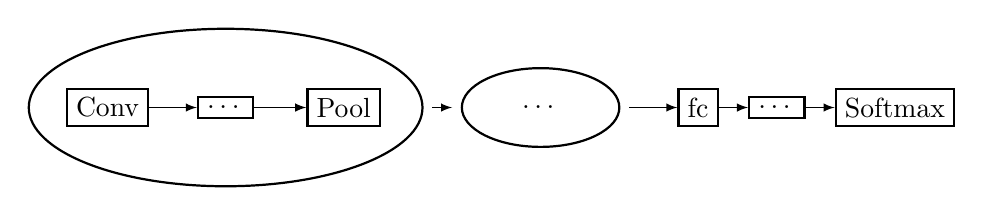
\begin{tikzpicture}
\tikzstyle{layer}=[rectangle, fill=white, thick, draw=black]
\node[layer] (C1) at (0,0) {Conv};
\node[layer] (CN) at (1.5,0) {\ldots};
\node[layer] (P1) at (3,0) {Pool};
\draw[thick, black] (1.5,0) ellipse (2.5 and 1);
\draw[thick, black] (5.5,0) ellipse (1 and 0.5);
\node[layer, draw=white] (CCN) at (5.5,0) {\ldots};
\node[layer] (FC) at (7.5,0) {fc};
\node[layer] (FCN) at (8.5,0) {\ldots};
\node[layer] (SM) at (10,0) {Softmax};
\node (AA) at (4,0) {};
\node (AB) at (4.5,0) {};
\node (AC) at (6.5,0) {};
\draw[-latex] (C1) to (CN);
\draw[-latex] (CN) to (P1);
\draw[-latex] (AA) to (AB);
\draw[-latex] (AC) to (FC);
\draw[-latex] (FC) to (FCN);
\draw[-latex] (FCN) to (SM);
\end{tikzpicture}
\caption[A general architecture of a convolutional neural network]{A general architecture of a convolutional neural network. The rectangles represent layers, \ldots represent optional repeating of previous layer. The ellipse is used to later illustrate possible repeating of a block of layers encapsulated in the ellipse}
\label{conv}
\end{figure}

\subsection{Architecture of used networks}

The networks used in our experiments were VGG16~\cite{vgg16} and ZFNet~\cite{zfnet}. The ZFNet network architecture is much smaller than the VGG16 network architecture -- the ZFNet architecture uses 5 convolutional layers with most of them directly followed by pooling layer while the VGG16 uses 13 convolutional layers but only 5 pooling layers altogether. Another important difference is that tha VGG16 network uses only convolutional layers with dimensions $3\times3\times n$ (with $n$ being variable according to previous layer output) and always having stride 1, while ZFNet uses convolutional layers with various dimensions and strides. The intermediate vector after the last pooling layer has size of 25088 for the VGG16 architecture while only 9216 for the ZFNet architecture.

The ZFNet is 8-layer architecture, where the original authors consider convolutional layer followed by pooling layer to count as 1 layer. The input layer expects images of dimension $224\times224\times3$ (where 3 stands for the RGB channels) and if the image we want to analyze does not fit this dimension, we simply scale it without keeping aspect ratio in order to fit. The first layer consists of 96 convolutional filters of size $7\times7\times3$ that have stride of 2 in $x$ and $y$ directions and stride 1 in $z$ direction. This feature map of dimension $110\times110\times96$ is then max-pooled by pooling window of size $3\times3$ and stride 2 to have output of the first layer of dimension $55\times55\times96$. The second layer consists of 256 filters of dimension $5\times5\times96$ while using stride 2 in $x$ and $y$ directions (and stride 1 in $z$ direction). The feature map of dimension $26\times26\time256$ is then again max-pooled by pooling window of size $3\times3$ and stride 2 in order to create the second layer's output of dimension $13\times13\times256$. The third layer consists of 384 convolutional filters of dimension $3\times3\times256$ with stride 1 in all directions and the fourth layer is essentially the same with 384 filters of size $3\times3\times384$ with stride 1 in all directions, therefore the feature map after fourth layer has dimension $13\times13\times384$. The fifth layer consists of 256 convolutional filters of dimension $3\times3\times384$ with stride 1 in all directions. The feature map is then max-pooled by pooling window of size $3\times3$ with stride 2 resulting in the feature map of dimension $6\times6\times256$. This feature map is then represented as a vector of size 9216 that is then fed into layers 6 and 7, each consisting of 4096 fully-connected neurons. The last layer is then $C$-way softmax function which essentially behaves as a fully connected layer with $C$ neurons, where $C$ is the number of classes to classify, directly followed by classical softmax function.

The VGG16 network architecture is one of the architectures presented in Simonyan's and Zisserman's paper introducing many experiments of different ConvNet network architectures. Variant 16 consists of 16 weighted layers, which was the second largest architecture in their series of experiments.

The architecture expects once again images of dimension $224\times224\times3$ and we use the scaling to achieve this dimension. The first two layers consist of 64 filters of dimension $3\times3\times3$ and $3\times3\times64$ respectively with stride 1 in all directions. After these two layers there is a max pooling layer with a window of size $2\times2$ and stride 2, such that after this layer the feature map has dimension $112\times112\times64$. Another two layers consist of 128 convolution filters of dimension $3\times3\times64$ and $3\times3\times128$ respectively with stride 1 in all directions and afterwards once again max pooling layer with a window of size $2\times2$ and stride 2 is applied such that the intermediate feature map has dimension $56\times56\times128$. Another 3 layers consist of 256 filters of dimension $3\times3\times128$ for the first layer and $3\times3\times256$ for the other two layers, all of them having stride 1 in all directions. Once again max pooling operation is present after this triple with a window of $2\times2$ and stride 2 to result in a feature map of dimension $28\times28\times256$. Next 6 layers consist of 512 filters for each layer, where the first one has dimension $3\times3\times256$ and other five have dimension $3\times3\times512$ with all filters having stride 1 in all directions. Max pooling layer is applied after first 3 layers of this 6-tuple and after the last layer, both of them having window of $2\times2$ and stride 2, resulting in a feature map of size $7\times7\times512$. This map is then fed as a vector of dimension 25088 into first next two fully-connected layers, each consisting of 4096 neurons each. Since the original paper~\cite{vgg16} was prepared for ILSVRC classification challenge which consist of 1000 different classes, last layer has 1000 fully-connected neurons, however this number is variable according to the number of classes to classify. The last layer is a simple softmax function.

All of the convolutional layers of both networks were directly followed by a ReLU unit.

\subsection{Faster \rcnn{} adjustments to network architecture} \label{rcnnarch}

When you want to run a detection and recognition pipeline, you are usually faced with a challenge of vast number of different positions and scales in which object you are interested might be in an image. Since passing an image through recognition network is quite time-consuming due to many computations in convolutional layers, many previous approaches tried to overcome this challenge with splitting this task into two different ones -- detection of Regions of Interest (RoI) and then classifying only a limited number of RoIs by convolutional networks. However since many computations between object detection and recognition can be shared, Faster \rcnn{}~\cite{faster} architecture merges those two computations back into one using a concept of Region Proposal Network which is a small extension of original recognition network. The RPN is put right before last pooling layer and consists of convolutional layer of size $3\times3$ (where width dimension is equal to width of preceding layer) and feeds the output of this layer into two sibling layers -- box-regression layer (\emph{reg}) and box-classification layer(\emph{cls}) which are both implemented as a convolutional layers of dimension $1\times1$. The \emph{reg} and \emph{cls} layers outputs $4k$ and $2k$ dimnesional vectors respectively, where $k$ stands for number of so called anchors at the processed position. Each anchor stands for a different setting of scales and aspect ratios at which RPN is analyzing given position. The original paper used three different scales and three different aspect ratios resulting in $k=9$. This approach ensures translational invariation of anchors. \emph{Reg} layer estimates regression of possible bounding box of an object and \emph{cls} layer computes 2 probabilities of object/not-object in each anchor at given position.

Outputs of this RPN network are then fed into Fast \rcnn{}~\cite{fast} part of networks, which expects RoI proposals and feature maps of last convolutional layer and applies so called RoI pooling effectively replacing last max pooling layer. RoI pooling divides each region of RoI proposal of dimension $w\times h$ into grid of size $W\times H$ where $W$ and $H$ are parameters of a layer (and in our experiments $W = H = 7$ was used) and performing classical max pooling on each cell of size $w/W\times h/H$ effectively squashing features of any RoI into fixed length vector of size $W\times H$.

This RoI pooled vector is then fed into usual fully-connected layers where the output at the end actually consists of two different output layers, one computing probability of a given class similarly as last layer of VGG16 or ZFNet networks and the other one estimating positions of bounding box depending on found class, therefore having $4C$ neurons where $C$ is number of classes to classify. Obviously the bounding box predictor is not followed by softmax layer.

\subsection{Training of a neural network} \label{train}

A general training algorithm for any neural network is usually done by evaluating the network on a training example and comparing the result of network with expected result by so called loss function. Loss function or error function is usually designed in a way that it measures by how much the result differs from the expected output and generally we try to minimize the output of such loss function over all training examples in a training set. This minimization can be seen as optimization problem and to solve this problem weights are adjusted in the direction of maximal gradient. This method is sometimes called as gradient descent algorithm.

Since deep networks have multiple layers, to adjust the weights of intermediate layers, the loss is then propagated backwards through the network by an algorithm called backpropagation which uses chain rule to iteratively compute gradients for each layer and adjust all of the weights in the network accordingly in attempt to minimize output of loss function. However, since the loss function $L$ is defined as the function of the weight settings $\textbf{w}$ over a dataset $S$ as sum of the loss function evaluated at each training example (equation \ref{loss}) and therefore computing gradient to compute new weights (equation \ref{grad}) for each training example is time consuming, stochastic gradient descent is usually used. We usually do not want to adjust the weights by the whole amount of gradient so learning rate $\alpha$ is used (often $\alpha\ll1$). $\textbf{w}_{t}$ denotes the weights of the network at an iteration $t$.

\begin{equation}
L(\textbf{w},S) = \sum_{i=1}^N L(\textbf{w},S_i)
\label{loss}
\end{equation}

\begin{equation}
\textbf{w}_{t+1} = \textbf{w}_{t} - \alpha\nabla L(\textbf{w}_{t},S) = \textbf{w}_{t} - \alpha\sum_{i=1}^N \nabla L(\textbf{w},S_i)
\label{grad}
\end{equation}

Stochastic gradient descent does essentially the same as classical gradient descent, however computes gradient only for one training example at a time and immediately after computing gradient of a loss function for one training example adjusts the weights accordingly. However since this is only an approximation, a good compromise between stochastic gradient descent and classical gradient descent is to use a minibatch of a reasonable size $n$ to adjust the weights according to gradient summed over $n$ random examples of the training set. In next equations, we will denote loss function as only a function of weights computed on a minibatch, $L(\textbf{w}) = \sum_{i=1}^n L(\textbf{w},S_n)$

One iteration usually adjusts the weights by a small amount so many iterations are still required.

Usually, other learning parameters different from learning rate are used as well. Most often used is momentum, $\mu$, that takes into account weight update of previous iteration under factor $\mu$ as well. Formal definition can be seen on equation \ref{momentum}, where $V_t$ denotes value by which weights are updated in iteration $t$ and $\textbf{w}_t$ denotes weights present in an iteration $t$.

\begin{equation}
\begin{array}{r c l}
V_{t+1}&=&\mu V_t - \alpha \nabla L(\textbf{w}_t)\\
\textbf{w}_{t+1}&=&\textbf{w}_t + v_{t+1}
\end{array}
\label{momentum}
\end{equation}

Another learning parameter often used is $\gamma$, used as a multiplier after a predefined number of iterations.

Caffe framework~\cite{caffe} allows you to set a multiplier of learning rate $\alpha$ for each layer used in your network. For convolutional and fully-connected layers, you can set them in \pyarg{param} part of layer definition, as \pyarg{param\{lr\_mult:x\}}, where $x$ is your desired $\alpha$. This feature is useful if you do not want to train your layers anymore and believe training only particular layers might be useful, you can set $\alpha$ for a particular layer to 0. Note however, that therefore the error will not propagate to preceding layers then.

Faster \rcnn{} needs to optimize for different loss functions -- two for RPN and two for classification and regression itself. The joint loss function for RPN is defined in equation \ref{rpnloss}, where $i$ is an index of an anchor in a minibatch, $p_i$ is predicted probability of the anchor $i$ being an object. The ground truth label $p^*_i$ is set to 1 for the anchor with highest intersection over union (IoU) with ground truth bounding box for a specific position out of $k$ anchors (as described in section \ref{rcnnarch}) and for each anchor having IoU with any ground truth box higher than 0.7. Note that this procudere may assign 1 to more anchors by a single ground truth bounding box. $t_i$ is parametrization of estimated bounding box, $t_i^*$ is parametrization of ground truth bounding box and $\lambda$ is balancing factor used in order to balance $L_{cls}$ and $L_{reg}$ for approximately the same amount of error. $\lambda$ was set to 10. As you can see, we computed loss function for \emph{reg} layer of RPN only when the RoI was actually an object ($p^*_i = 1$). $L_{cls}(p,p^*)$ is a classical logarithmic loss function $L_{cls}(p,p^*) = -p^*\log(p)$ and $L_{reg}(t,t^*)$ is a smooth $L_1$ loss of a $t_i - t_i^*$. The parametrization of bounding boxes can be seen on equation \ref{param}, $x$, $y$, $w$ and $h$ denote center coordinates of estimated bounding box, its width and height, $x_a$, $y_a$, $w_a$ and $h_a$ denote the same properties for anchor box and $x^*$, $y^*$, $w^*$ and $h^*$ denote the same properties for ground truth box.

\begin{equation}
L_{RPN}(\{p_{i}\}, \{t_{i}\}) = \frac{1}{N}\sum_{i=1}^{N}L_{cls}(p_{i}, p^*_{i}) + \lambda\frac{1}{N}\sum_{i=1}^{N}p^*_{i}L_{reg}(t_{i},t^*_{i})
\label{rpnloss}
\end{equation}

\begin{equation}
\begin{array}{c c c c}
t_x = (x- x_a)/w_a & t_y = (y-y_a)/h_a & t_w=\log(w/w_a) & t_y=\log(h/h_a)\\
t_x^* = (x^* - x_a)/w_a & t_y^* = (y^* - y_a)/h_a & t_w^*=\log(w^*/w_a) & t_y^*=log(h^*/h_a)
\end{array}
\label{param}
\end{equation}

Smooth $L_1$ loss function is then defined on equation \ref{smooth}.

\begin{equation}
\text{smooth}_{L_1}(x) = \left\{
\begin{array}{ll}
0.5x^2 & \mbox{if } |x| < 1 \\
|x| - 0.5 & \mbox{otherwise}
\end{array}
\right .
\label{smooth}
\end{equation}

The same loss function is used for classification and regression itself with slight change in $L_{reg}$. $L_{reg}(b_i,b_i^*)$ for prediction of bounding boxes does not know anything about the anchors anymore and therefore the function is defined in equation \ref{reg}. SGD Solver implemented in Caffe is able to optimize network for multiple loss functions and therefore we can start training with these two loss functions defined.
\begin{equation}
L_{reg}(b_i,b^*_i) = \sum_{j\in\{x,y,w,h\}}\text{smooth}_{L_1}(b_{ij} - b_{ij}^*)
\label{reg}
\end{equation}

\section{Precision-recall curve}
Precision recall-curve can be used to visualize performance of binary classification task. Let's define four variables -- $TP$, $TN$, $FP$ and $FN$. $TP$ is a number of examples that were correctly classified with desired label, $TN$ is a number of examples, that were correctly not classified -- desired label was not present in ground truth and classification tool did not assign it a label, $FP$ is number of examples where label was not present in ground truth, but classification tool assign this example a label and $FN$ is a number of examples where label present was present in ground truth but classification tool did not assign it a label. After these definition, it is possible to define precision as a fraction of correctly classified examples out of examples, that were assigned a label (equation \ref{prec}) and recall as a fraction of correctly classified examples out of examples, that should have been assigned a label (equation \ref{recall}).

\begin{equation}
\text{precision} = \frac{TP}{TP+FP}
\label{prec}
\end{equation}
\begin{equation}
\text{recall} = \frac{TP}{TP+FN}
\label{recall}
\end{equation}

However, these definitions hold valid only for binary classifications. To create a precision-recall curve for a recognition task with one class whose output is a probability, it is possible to be incrementally setting a probability threshold which then acts as borderline between assigning a label and not assigning a label. To extend this for more classes at once, it is possible to treat the assignment of the class $C_1$ to the ground truth class $C_2$ as both $FP$ and $FN$ since the class $C_1$ was assigned to example which did not have the ground truth class $C_2$ and there was no class $C_2$ label assigned to the ground truth class $C_2$ although it should be.

The goal is to achieve as high precision as possible with as high recall as possible.
